\section{Introduction}
\label{sec:intro}
This report will discuss the notebook we made on restricted Hartree-Fock theory.
We will walk trough the notebook step by step and discuss what we see there. 
The same titles as in the notebook will be used, as to make sure the report can be 
easily followed. Relevant parts of the code will be displayed.

 \section{Theoretical Approach}
 \label{sec:theory}
 \subsection{Introduction to Theory}
 \label{subsec:intro}
 Before we actually dive into the code, we will discuss the theory behind it.
 The actual goal of this experiment is to calculate the energy of a molecule,
 mainly to solve the Schrödinger equation for that molecule. This, unfortunately,
is impossible. The interelectronic interactions prohibit us from separating the variables.
Intuitvely, we would need the coordinates of the second electrons to determine the
coordinates of the second electron. But for those, we would need the coordinates of
the first electron again. So we have to find an alternative. This alternative would be
Hartree-Fock theory. Bluntly put we can define another operator, the Fock operator,
that consists of one-electron operators and two-electron operators. This is 
displayed in Equation \ref{eq: fock matrix}. 

\begin{equation}\label{eq: fock matrix}
    \hat{f}(1) = \hat{h}(1) + 2\sum_i^{N/2}\hat{J}_i - \sum_i^{N/2}\hat{K}_i
\end{equation}
$\hat{h}$ is a one electron Hamiltonian, which accounts for the kinetic energy of
the electron and the potential energy with respect to the nucleus. $\hat{J}$ is the Coulomb operator, it accounts for the interelectronic repulsion. 
$\hat{K}$ is the exchange operator, that accounts for the stabilizing interaction between 
electrons that have the same spin. 
\subsection{Deriving the Fock Operator}
\label{subsec:fock matrix}
Let us step back a bit here to see where this operator comes from. To do that, we 
need to begin with the true Hamiltonian for the system, which is given in Equation 
\ref{eq:hamilthe}
\begin{equation}\label{eq:hamilthe}
    \hat{\boldsymbol{H}} = \sum_i^N\hat{h}(i) + \frac{1}{2}\sum_i^N\sum_j^N\frac{1}{|\boldsymbol{r}_i - \boldsymbol{r}_j|}
\end{equation}
$\hat{h}(i)$ is a one electron operator, as said before. The second term accounts 
for interelectronic interactions. $|\boldsymbol{r}_i - \boldsymbol{r}_j|$ is 
merely the distance between electrons $i$ and $j$. Now, we also need a 
wavefunction $\Psi$, which is a Slater determinant. This determinant looks like 
Equation \ref{eq:slater}.
\begin{equation}\label{eq:slater}
    \ket{\Psi} = 1/\sqrt{N!}\begin{vmatrix}
        \chi_1(\boldsymbol{x}_1) & \cdots & \chi_n(\boldsymbol{x}_1) \\
        \cdots & \cdots & \cdots \\
        \chi_1(\boldsymbol{x}_n) & \cdots & \chi_n(\boldsymbol{x}_n)\\
    \end{vmatrix}
\end{equation}
When we look at the individual functions $\chi_i(\boldsymbol{x}_j)$ we can state Equation 
\ref{eq:spinor}

\begin{equation}\label{eq:spinor}
    \chi_i(\boldsymbol{x_j}) = \psi_i(\boldsymbol{r}_j)\gamma(\boldsymbol{\omega}_j)
\end{equation}
Here, $\psi$ is a spatial orbital, $\gamma$ is a spin function, which can be either
$\alpha$ or $\beta$. Now we have all the ingredients, we can start building the Fock
matrix. The first step would be to calculate the expectation value of the 
Hamiltonian over the wave function $\Psi$. First of all we assert that all spin-orbitals
are normalised, so that $\braket{\chi_i}{\chi_i} = 1$. We will not give the exact 
derivation here, but jump straight to the end result. This is given in Equation 
\ref{eq:expect}.

\begin{multline}\label{eq:expect} 
    \bra{\Psi}\hat{\boldsymbol{H}}\ket{\Psi} = \sum_i^N\bra{\chi_i}\hat{h}(1)\ket{\chi_i} + \frac{1}{2}\sum_i^N\sum_j^N\left(\int\chi_i^*(1)\chi_i(1)\frac{1}{|\boldsymbol{r}_i- \boldsymbol{r}_j|}\chi_j^*(2)\chi_j(2)d1d2 \right.\\
     \left. - \int\chi_i^*(1)\chi_j(1)\frac{1}{|\boldsymbol{r}_i - \boldsymbol{r}_j|}\chi_j^*(2)\chi_i(2)d1d2\right)
\end{multline}
This expectation value can always be calculated, even if $\Psi$ is not an eigenfucntion
of the Hamiltonian. The only problem we have here is the choice of the spin-orbitals.
We need to choose them in such a way that the energy is minimal. This would mean
that the energy is a stationary point, so we enforce Equation \ref{eq:condition}.  
\begin{equation}\label{eq:condition}
    E(\chi_i + \delta\chi_i) - E(\chi_i) =\delta E = 0
\end{equation}
E is off course nothing else then the expectation value of the
wave function $\Psi$ over the Hamiltonian. We could write $\bra{\Psi}\hat{\boldsymbol{H}}\ket{\Psi} = E(\chi_i)$. 
Now we will enforce orthonormality of the spin-orbitals via a seperate function, as
can be seen in Equation \ref{eq:lagrange}.
\begin{equation}\label{eq:lagrange}
    L = E - \sum_{ij}\epsilon_{ij}(\braket{\chi_i}{\chi_j} - \delta_{ij})
\end{equation}
This is another constraint we need to enforce, since whatever fucntions we are 
looking for, they need to be orthonormal. If they are not, we need to make a correction.
This is done by introducing the fucntion L. It is easy to see that in the case of
orthonormal spin-orbitals L reduces to E. The $\epsilon_{ij}$ are the Lagrange 
multipliers. Now we will calculate $\delta L$, this is possible with the 
information that is given. We will once again skip to the end. The final equation 
is given in Equation \ref{eq:deltaL}.
\begin{equation}\label{eq:deltaL}
    \delta L = \sum_i\bra{\delta\chi_i}\hat{h}(1) + \sum_j(\hat{J_j} - \hat{K_j})\ket{\chi_i} -  \sum_{ij}\epsilon_{ij}\braket{\delta\chi_i}{\chi_j} + complex\:conjugate = 0
\end{equation}
We have added the Coulomb and exchange operators. When we define the expectation
values as Equations \ref{eq:coulomb} and \ref{eq:exchange}, we see that we can indeed
add them in this way.

 \begin{equation}\label{eq:coulomb}
    \bra{\chi_i}\hat{J}_j\ket{\chi_i} = \int\chi_i^*(1)\chi_j^*(2)\frac{1}{|\boldsymbol{r}_i- \boldsymbol{r}_j|}\chi_i(1)\chi_j(2)d1d2
 \end{equation}

 \begin{equation}\label{eq:exchange}
     \bra{\chi_i}\hat{K}_j\ket*{\chi_i} = \int\chi_i^*(1)\chi_j(1)\frac{1}{|\boldsymbol{r}_i - \boldsymbol{r}_j|}\chi_j^*(2)\chi_i(2)d1d2)
 \end{equation}
When we check Equation \ref{eq:deltaL}, we see that it can only hold if Equation \ref{eq:fockeqpreq}
and its counterpart from the complex conjugate both hold.

\begin{equation}\label{eq:fockeqpreq}
    \left(\hat{h}(1) + \sum_j(\hat{J_j} - \hat{K_j})\right)\chi_i = \sum_{j}\epsilon_{ij}\chi_j
\end{equation}
These two equations allow us to conclude that $\epsilon^*_{ij} = \epsilon_{ji}$.
These factors are called the Lagrange multipliers and form a Hermitian matrix. 
When we take a closer look at the operator in Equation \ref{eq:fockeqpreq}, we 
can recognise the Fock operator from Equation \ref{eq: fock matrix}, although
we are not quite there yet. However we can already write some interesting equations
with the formulas we have. We can write Equation \ref{eq:fockeq}.

\begin{equation}\label{eq:fockeq}
    \hat{f}(1)\chi_i = \epsilon_i\chi_i
\end{equation}
These equations are called the Hartree Fock equations.
\subsection{Restricted Hartree-Fock}
\label{subsec:RHF}
As we said in the last subsection, we are not quite where we want to be just yet.
We need to get to the Fock matrix from Equation \ref{eq: fock matrix}, but we are
only at the one in \ref{eq:fockeqpreq}. This is where we will make the jump to
restricted Hartree Fock theory. To start, we will take a look at Equation \ref{eq:spinor}.
Here we saw that the spin-orbital is actually a product of a spatial orbital and
a spin function. When we take a look at our operators however, we notice that none
of them will actually interact with this spin function. We would then like to get rid
of it. Doing this is actually not that difficult. If we would collect all functions
that have $\alpha$ as their spin component, we can write a Hartree-Fock equation and
then simply integrate the spin component out by adding $\bra{\alpha}$ on every
side of the equation. For the one electron part and the Coulomb operators, there is
no problem at all, since all electrons stay in their respective orbitals. However,
the exchange operator will move electrons around to different spin-orbitals.(see 
Equation \ref{eq:exchange}) When the electron from an $alpha$ spin-orbital would
be moved to a $beta$ spin-orbital, this would result in a zero, since $\bra{\alpha}\ket{\beta} = 0$
So here it is clear that the exchange operator will only remain active after spin 
elimination between electrons that have the same spin function. So now that we have
gotten rid of spin, all that is left is Equation \ref{eq:spinelim}.

\begin{equation}\label{eq:spinelim}
    \hat{f}^{\alpha}(1)\psi^{\alpha}_i = \epsilon^{\alpha}_i\psi^{\alpha}_i
\end{equation}
Off course the same argument stands for the $\beta$-spins.

Now we have come to a point where we can define a restricted closed shell system.
Imagine what would happen if all orbitals were doubly occupied, with an $\alpha$
and a $\beta$ electron, all according to the Pauli princple. This has some consequences.
The first one is that the amount of $\alpha$-electrons would equal the amount of
$\beta$-electrons. Secondly, this would mean that the difference between these electrons
is only their spin function. They reside in the same orbitals. This means that we only
need to account for half the electrons, since the other half is in the same orbitals,
just with a different spin. Now think about the Fock operator. Let us
take a look at a single electron. It has a one election hamiltonian, electronic repulsion
for all other electrons in the system and it only "exchanges" with half of the other
electrons, only those with the same spin. This means we have a double the amount of 
Coulomb operators to exchange operators. When we now look back at Equation \ref{eq: fock matrix},
we see that we are finally there.

\subsection{Application of the Hartree-Fock Theory}
\label{subsec:applic}
At this point, we might think back to the point where we defined the Coulomb and
exchange operators. These operators themselves depend on the orbitals. So we would
need to know the orbitals to define our operator. It seems we are stuck again.
However we can apply some mathemathical tricks to get us out of this impasse. 
First we can assert that every function can be expressed as a linear combination
of basis functions. We also know that the eigenfunctions of a Hermitian operator
form such a set of basis functions. We begin by selecting a convenient basis set.
This could be a set of atomic orbitals. Then we would solve the eigenproblem in
Equation \ref{eq:eigenproblem}.

\begin{equation}\label{eq:eigenproblem}
    \boldsymbol{\hat{H}}^{core}\boldsymbol{C} = \boldsymbol{SC}c
\end{equation} 
C is a coeficcient matrix. It holds the coeficcients of the eigenfunctions of the
Hamilonian (or later the fock operator) in the basis. Calculating the eigenvalues 
and eigenfunctions for the core Hamiltonian is perfectly possible, since it is a 
one-electron operator. We now have a set of orbitals which we can use to build 
our Fock operator. For this Fock operator, we can solve the generalised 
eigenproblem in the form of the Roothaan-Hall equations 
(see Equation \ref{eq:Roothaan-Hall}).

\begin{equation}\label{eq:Roothaan-Hall}
    \boldsymbol{FC} = \boldsymbol{SC}\epsilon
\end{equation}

Solving this equation will give us a set of eigenfunctions of the Fock matrix. 
These functions can then be used to build a new Fock matrix. This is where we 
start the iterations. We can continue untill we reach a point where the energy 
does not change any more. At that point, we have found the energy of the molecule.

Before we move on, some clarifications are in order. 
\begin{enumerate}
    \item The basis set we choose is not the same as the set that is derived
    from the eigenfunctions of the Hamiltonian. These eigenfunctions are in fact
    our first guess of the actual molecular orbitals. However, this guess will not be
    very good yet, since of course the core Hamiltonian is not the same as the 
    molecular Hamiltonian. 
    \item A basis set is often chosen for the ease of integration. Often, these
    are Gaussian functions. So we can see that the chosen basis set does not
    need to have the same properties as the eigenfunctions of the Hamiltonian. 
    Of course the functions do have to be "well-behaved". The size however, will always be the same.
    If you choose a basis set with only two functions, your Hamiltonian will have only
    two eigenfunctions. The bigger the basis set, the more eigenfunctions you will have. 
    \item We are using an expansion of a function in a basis. That is always possible.
    However, there is always a catch, namely that the basis set used has to be complete.
    In most cases this would actually mean that it is infinitely large, so of no
    real use to us. However, if we choose an incomplete set, we will only be able
    to make approximations.
    \item If we want to do the expansion, we need to integrate the spin out first.
    So we need to end up with an expansion that is only dependent on the spacial
    orbital, like in Equation \ref{eq:expansion}.
    \begin{equation}\label{eq:expansion}
        \psi_i = \sum_jC_{ji}\phi_j
    \end{equation}
\end{enumerate}

\subsection{The Density Matrix}
\label{subsec:theDM}
At this point we still need to adress one topic, the density matrix. This will be
very important since it will be used to calculate the Fock matrix in our program.
To demonstrate what it is, we will look at the expression for the Coulomb operator.
When we take Equation \ref{eq:coulomb} and then expand the functions $\chi_i$ in
a basis after eliminating the spin, we find Equation \ref{eq:coulombexp}.

\begin{equation}\label{eq:coulombexp}
    \hat{J}_i = \int\sum_{\sigma}C^*_{\sigma}\phi^*_{\sigma}(x_j)\frac{1}{|\boldsymbol{r}_1 - \boldsymbol{r}_j|}\sum_{\nu}C_{\nu}\phi_{\nu}(x_j)dx_j
\end{equation}

The C factors in this equation are merely the exapansion coeficcients of the function
$\psi_i$.(Rememmber that this is the spatial orbital, see Equation \ref{eq:spinor})
These are constants, so we can safely extract them from the integrals to form
Equation \ref{eq:coulombexp1}.

\begin{equation}\label{eq:coulombexp1}
    \hat{J}_i = \sum_{\sigma}\sum_{\nu}C_{\nu j}C^*_{\sigma j}\int\phi^*_{\sigma}(x_j)\frac{1}{|\boldsymbol{r}_1 - \boldsymbol{r}_j|}\phi_{\nu}(x_j)dx_j
\end{equation}
We can apply this same strategy to the exchange operator. In the end we will be
able to factor out the products of the expansion coëficcients and afer summation
over all basis functions we can define the density matrix as Equation 
\ref{eq:densitymatrix}.

\begin{equation}\label{eq:densitymatrix}
    D_{\sigma\nu} = 2\sum^{N/2}_jC_{\sigma j}^*C_{\nu j}
\end{equation}
This will be used to calculate the Fock matrix. (see below). However, before we 
move on, there is something noteworthy here. We only have to account for the 
occupied orbitals $j$. Let us take the example where there are seven eigenfucntions
and only ten electrons. In restricted closed shell Hartree Fock that would mean
five doubly occupied orbitals. We would only have to consider the five occupied
orbitals here. You would still end up with a seven by seven density matrix. This
can be seen more clearly in Section \ref{sec:step3}.

\section{Identifying the Molecule}
\label{sec:step1}
In this first step we initiated the class molecule, which will be equipped with 
the necessary methods to do all the calculations we will be required to do. 
A molecule object has several properties that need to be defined first. 


\begin{python}[caption={intitialising the molecule object},label={ls:Listing 1}]
    class molecule:
        def __init__(self, geom_file):
            if """pubchem""" in geom_file:
                self.id = psi4.geometry(geom_file)
            else:
                self.id = psi4.geometry(f"""
                {geom_file}
            
                units bohr
                """)
            self.id.update_geometry()
            self.wfn =  psi4.core.Wavefunction.build(self.id, 
                            psi4.core.get_global_option('basis'))
            self.basis = self.wfn.basisset()
            self.integrals = psi4.core.MintsHelper(self.basis)
            # only works for closed shell systems
            self.occupied = self.wfn.nalpha()  
            self.guessMatrix = "empty"
    
\end{python}
  

In Listing \ref{ls:Listing 1} we define the \pythoninline{__init__} method of the 
molecule class. It sets us up with some of the information we will need later, 
namely the \pythoninline{psi4.core.Molecule} representation as 
\pythoninline{self.id}. We also see the wave function, basis set, 
integrals, occupied orbitals and a guess matrix. 
Since we will be doing Hartree-Fock calculations, which involve a 
lot of iterations, the molecule object will need a way to store the Fock 
matrix from the last iteration. From there we can then start for the next 
iteration. Hence, the first method we actually have to define is a method that 
allows us to change this parameter.


\begin{python}[caption={setting the guessMatrix},label={ls:Listing 2}]
    def setGuess(self, new_guess):
        """
        sets the guessMatrix to a new value

        input:
        new_guess: numpy array that represents a new fock matrix
        """
        self.guessMatrix = new_guess
\end{python}

This is shown in Listing \ref{ls:Listing 2}. 

\section{Prerequisite Calculations}
\label{sec:step2}

In this section, we do some prerequisite calculations. These are relatively 
straightforward. In this step, we added some methods to the class that allow us to 
calculate important properties like the nuclear repulsion, kinetic energy and so 
on. The commands used are directly implemented from the psi4 package. 
They are listed in Table \ref{tab:commands}

\begin{table}[H]
    \centering
    \begin{tabular}{c|c}
        command & property \\
        \hline
        \pythoninline{self.id.nuclear_repulsion_energy()}| & nuclear repulsion energy \\
        \pythoninline{self.integrals.ao_overlap().np} & overlap matrix \\
        \pythoninline{self.integrals.ao_kinetic().np} & kinetic energy \\
        \pythoninline{self.integrals.ao_potential().np} & potential energy \\
        \pythoninline{self.displayE_kin() + self.displayE_pot()} & the core hamiltonian \\
        \pythoninline{self.integrals.ao_eri().np} & repulsion between electrons \\
    \end{tabular}
    \caption{Commands useed to calculate various properties}
    \label{tab:commands}
\end{table}
We will not list the code for the various methods here, however when they appear
 in later blocks of code we will mention them.

\section{The inital (Guess) Density Matrix}
\label{sec:step3}
We will skip ahead to the function that gives us the density matrix and start
 from there.

 
\begin{python}[caption={calculating the density matrix},label={ls:Listing 3}]
        class molecule(molecule):
            def getDensityMatrix(self):
                """
                generates the densitiy matrix on the AO level
                """
                C = self.getEigenStuff()[1]
                A = 2*np.einsum("pq, qr->pr", C[:, :self.occupied], 
                                C[:, :self.occupied].T, optimize=True)
                return A
\end{python}

This function uses the method \pythoninline{getEigenStuff}, which just calls 
the scipy function \pythoninline{linalg.eigh}. This solves the generalised 
eigenproblem posed by the Roothaan-Hall equations, Equation \ref{eq:Roothaan-Hall}, 
for whatever matrix that is currently in the \pythoninline{self.guessMatrix} 
parameter. C in Listing \ref{ls:Listing 3} then refers to \textbf{C} in Equation 
\ref{eq:Roothaan-Hall}. The first matrix for which we calculate the eigenvalues 
and eigenvectors is the core Hamiltonian, so this will have to be stored as the 
\pythoninline{self.guessMatrix} before proceeding. Now we are set to build a Fock 
matrix.

\section{Updating the Fock Matrix}
\label{sec:step4}


    
\begin{python}[caption={calculating the Fock matrix},label={ls:Listing 4}]
    class molecule(molecule):
        def displayFockMatrix(self):
            """Will display the Fock matrix"""
            coulomb = np.einsum("nopq,pq->no", 
                    self.displayElectronRepulsion(), 
                    self.getDensityMatrix(), optimize=True)
            exchange = np.einsum("npoq,pq->no", 
                    self.displayElectronRepulsion(), 
                    self.getDensityMatrix(), optimize=True)
            self.fockMatrix = self.displayHamiltonian() 
                            + coulomb - 0.5*exchange
            return self.fockMatrix
\end{python}
 
 
We see that the Fock-matrix uses the density matrix and the electronic 
repulsion matrix and the Hamiltonian , which the molecule object calls with the 
methods seen in Section \ref{sec:step2}. Since the density matrix depends on the 
current \pythoninline{self.guessMatrix}, the Fock matrix will also depend on it. 
We will discuss the importance of this in Subsection \ref{subsec: iteration}. 

 
 \section{The SCF Energy}
 \label{sec:step5}
 From the Fock matrix we derived in the previous section, we can now calculate 
 the electronic energy according to Equation \eqref{eq:energy}.
 
 \begin{equation} \label{eq:energy}
     E_{elek} = \frac{1}{2}\sum_{\mu\nu}D_{\mu\nu}\cdot(H_{\mu\nu} + F_{\mu\nu})
 \end{equation}
 In Python this looks like Listing \ref{ls:Listing 5}.
 
 
    
\begin{python}[caption={calculating the energy},label={ls:Listing 5}]
    class molecule(molecule):
        def getElectronicEnergy(self):
            """
            calculates the energy with the current fock matrix
            """
            sumMatrix = self.displayHamiltonian() 
                    + self.displayFockMatrix()
            return 0.5*np.einsum("pq,pq->", sumMatrix, 
                            self.getDensityMatrix())
\end{python}

The total energy is merely the sum of this electronic energy and the nuclear 
repulsion energy. We have a method for the latter defined in Section 
\ref{sec:step2}.
 
 \section{Test for Convergence}
 \label{sec:step6}
Now we only need to bring this all together to get the final energy. 
This is done in the function \pythoninline{iterator} as seen in Listing 
\ref{ls:Listing 6}.

 
   
\begin{python}[caption={iteration sequence},label={ls:Listing 6}]
    def iterator(target_molecule):
        """
        Function that performs the Hartree-Fock iterative calculations 
        for the given molecule.
        
        input:
        target_molecule: a molecule object from the class molecule
        """
        # setting up entry parameters for the while loop
        E_new = 0  
        E_old = 0
        d_old = target_molecule.getDensityMatrix()
        convergence = False
        E_list = []

        # step 2: start iterating
        itercount = 0
        while not convergence and itercount < 50:

            # calculating block: calculates energies
            E_new = target_molecule.getElectronicEnergy()
            E_total = target_molecule.getTotalEnergy()

            # generating block: generates new matrices
            F_n =  target_molecule.displayFockMatrix()
            target_molecule.setGuess(F_n)
            d_new = target_molecule.getDensityMatrix()

            # comparing block: "Are we there yet?"
            rms_D = np.einsum("pq->", np.sqrt((d_old - d_new)**2))
            if abs(E_old - E_new) < 1e-6 and rms_D < 1e-4:
                convergence = True


            # maintenance block: keeps everything going
            print(f"""iteration: {itercount}, E_tot: {E_total: .8f}, 
                        E_elek: {E_new: .8f}, 
                        deltaE: {E_new - E_old: .8f}, 
                        rmsD: {rms_D: .8f}""")
            E_old = E_new
            d_old = d_new
            E_list.append(E_new)
            itercount += 1
        
        return E_list
\end{python}

First we need to set up the parameters before we start iterating. That is done in 
the first block of code. Then we start a while loop, that will stop iterating once
we have reached convergence, or when we have reached the maximum amount of 
iterations. Inside the loop, we see four blocks of code. The calculating block 
provides us with the energy of the molecule for the given 
\pythoninline{self.guessMatrix}. The next block will generate new matrices for 
the next iterative step. In the comparing block we check the conditions for 
convergence. For this we need four values, the old and new energies and the old 
and new distance matrices. For more information, see Subsection 
\ref{subsec:step6.1}. For now we will continue to walk trough the code. 
After the comparing block we move to the final block, which sets us up for the 
next iteration. This iterations energy is stored, as well as the density matrix. 
We print out a line that summarises all the relevant values for this iteration. 
We can then move on to the next iterative step until the while loop finds one of 
its conditions is no longer met.

\subsection{On Iterations and the Molecule Object}
\label{subsec: iteration}
In this subsection we will discuss what the iteration actually does to the 
molecule object along the way. We call a lot of methods on the object, but those 
do not change any of the fundamental properties of the object. Now pay special
attention to the generating block, where we change the 
\pythoninline{self.guessMatrix} to a new value. After this is done, all new values
that are calculated will be based on the new matrix. This is the only value that 
actually changes, but is has far reaching consequences on all the methods. 

 
 \subsection{On Comparing Values}
 \label{subsec:step6.1}
In Listing \ref{ls:Listing 6} we can see that there is a difference in the
citeria for the density matrix and the energy. However when we look at the 
equation we see that the energy uses the density matrix. Indeed we see in 
Equation \ref{eq:energy} that the energy is calculated using a 
product of the Fock matrix with the density matrix, which already uses the density
matrix as can be seen in Equation \ref{eq: fock-matrix}.
 
 \begin{equation} \label{eq: fock-matrix}
     F_{\mu\nu} = H_{\mu\nu} + \sum^{AO}_{\lambda\sigma}D_{\lambda\sigma}[(\mu\nu|\lambda\sigma) - \frac{1}{2}(\mu\lambda|\nu\sigma)]
 \end{equation}

Considering that the root-mean-square of the density matrix uses all elements of 
this matrix, we could say that the criterion for the density matrix is inherently
the strictest, since the energy criterion only uses one single value and the 
density matrix criterion uses a multitude of values that have to behave 
accordingly. However, this expalanation is to simple. Since the energy uses 
the density matrix, these conditions are in fact connected. In this case that 
would mean that enforcing one condition is enough to enforce the other one. 
We can indeed see that this is the case in Section \ref{sec: examples}. 

 
 \section{Some examples}
 \label{sec: examples}
 In this section, we will display some of the results from our calculations for 
 two example systems, water and methane. We will give a display of the output as 
 generated by the functions we discussed above.
 
 \subsection{water}
 \label{subsec:water}

\begin{python}[caption={iterations for water},label={ls:Listing 7},basicstyle=\scriptsize]
0, E_tot: -73.28579642, E_elek: -81.28816348, deltaE: -81.2881634, rmsD:  14.05298222
1, E_tot: -74.82812538, E_elek: -82.83049244, deltaE: -1.54232896, rmsD:  3.17285816 
2, E_tot: -74.93548800, E_elek: -82.93785506, deltaE: -0.10736262, rmsD:  0.65858574 
3, E_tot: -74.94147774, E_elek: -82.94384480, deltaE: -0.00598974, rmsD:  0.24093051 
4, E_tot: -74.94197200, E_elek: -82.94433906, deltaE: -0.00049425, rmsD:  0.08612099
5, E_tot: -74.94205606, E_elek: -82.94442312, deltaE: -0.00008407, rmsD:  0.04061885
6, E_tot: -74.94207442, E_elek: -82.94444148, deltaE: -0.00001836, rmsD:  0.01827516
7, E_tot: -74.94207865, E_elek: -82.94444571, deltaE: -0.00000423, rmsD:  0.00892060
8, E_tot: -74.94207963, E_elek: -82.94444669, deltaE: -0.00000098, rmsD:  0.00425406
9, E_tot: -74.94207986, E_elek: -82.94444692, deltaE: -0.00000023, rmsD:  0.00205358
10, E_tot: -74.94207991, E_elek: -82.94444697, deltaE: -0.00000005, rmsD:  0.00098889
11, E_tot: -74.94207992, E_elek: -82.94444699, deltaE: -0.00000001, rmsD:  0.00047710
12, E_tot: -74.94207993, E_elek: -82.94444699, deltaE: -0.00000000, rmsD:  0.00023011
13, E_tot: -74.94207993, E_elek: -82.94444699, deltaE: -0.00000000, rmsD:  0.00011102
14, E_tot: -74.94207993, E_elek: -82.94444699, deltaE: -0.00000000, rmsD:  0.00005356
\end{python}
Here we see the the amount of iterations before the convergence is reached and 
all parameters calculated during that iteration. Furtermore we can use the 
\pythoninline{oeprop} method to get the dipole and nuclear charges. The dipole 
moment is given in e\AA, the charge is given in e, where e is the elemental 
charge.

\begin{table}[ht]
    \centering
    \begin{tabular}{c|c}
         total dipole moment & 0.6034  \\
         \hline
         nuclear charges &  \\ 
         \hline
         O & -0.25302 \\
         H & 0.12651 \\
         H & 0.12651 \\
    \end{tabular}
    \caption{Some properties of water}
    \label{tab:number2}
\end{table}

\begin{figure}
    \centering
    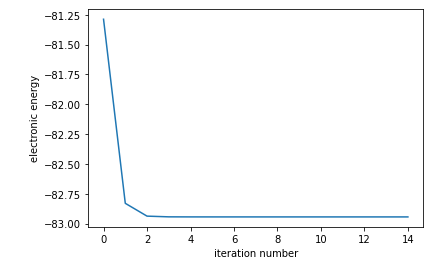
\includegraphics[width=0.5\textwidth]{content/Capture.PNG}
    \caption{convergence for water}
    \label{fig:convergence1}

\end{figure}
\subsection{methane}
\label{subsec:methane}
 
\begin{python}[caption={iterations for methane},label={ls:Listing 8},basicstyle=\scriptsize]
0, E_tot: -36.08344857, E_elek: -49.58075304, deltaE: -49.58075304, rmsD:  35.9980315
1, E_tot: -39.56451342, E_elek: -53.06181788, deltaE: -3.48106485, rmsD:  4.73662689
2, E_tot: -39.72183632, E_elek: -53.21914079, deltaE: -0.15732290, rmsD:  0.79654919
3, E_tot: -39.72669300, E_elek: -53.22399746, deltaE: -0.00485667, rmsD:  0.14041648
4, E_tot: -39.72684535, E_elek: -53.22414982, deltaE: -0.00015236, rmsD:  0.02394664
5, E_tot: -39.72685016, E_elek: -53.22415462, deltaE: -0.00000480, rmsD:  0.00443984
6, E_tot: -39.72685031, E_elek: -53.22415477, deltaE: -0.00000015, rmsD:  0.00072904
7, E_tot: -39.72685032, E_elek: -53.22415478, deltaE: -0.00000001, rmsD:  0.00014205
8, E_tot: -39.72685032, E_elek: -53.22415478, deltaE: -0.00000000, rmsD:  0.00002652
\end{python}
 
 \begin{table}[ht]
    \centering
    \begin{tabular}{c|c}
         total dipole moment & 0.0000  \\
         \hline
         nuclear charges &  \\ 
         \hline
         C & -0.26031 \\
         H & 0.06508 \\
         H & 0.06508 \\
         H & 0.06508\\
         H & 0.06508 \\
    \end{tabular}
    \caption{Some properties of methane}
    \label{tab:number2}
\end{table}

